%%%%%%%%%%%%%%%%%%%%%%
\section{Extensibility Discussion}
%%%%%%%%%%%%%%%%%%%%%%

\subsection{Optimizations to Current Design}\label{sec:optimizations}
The design that we propose in this paper demonstrates that it is feasible to build a 10 Gb/s line rate PIFO scheduler on an FPGA. However, we would like to point a potential optimization that would allow the design to scale to support even higher line rates.

\subsubsection*{Pipelined skip list operation}
Pipelining is the concept of partitioning logic into discrete stages to allow subsequent operations to begin processing before previous operations have fully completed. This is a common design technique that is used when designing line rate systems. For example, the authors of \cite{pipelined-heap-2007} use this approach to build a 10Gb/s pipelined heap for ASICs. The design techniques that we use in this paper, namely parallelism and a small-fast sorting cache, challenge the conventional wisdom that line rate systems must make use of heavy pipelining. Note that these techniques are completely orthogonal. We can improve the performance of our skip list implementation by pipelining the required operations. This would allow enqueue operations to occur more frequently and hence reduce the number of priority queues that must be used in parallel.

The key to building a pipelined system is to identify discrete stages of logic that perform approximately the same amount of work. For a deterministic skip list, it is natural to divide the processing of each level into individual stages. All of the nodes belonging to a particular level can be stored in a separate BRAM, as shown in Figure \ref{fig:pipe-skip-list}. Each stage then has some fixed number of clock cycles to complete the processing on the nodes in that level. Fortunately, the deterministic skip list bounds the number of memory operations that are required at each level so it is possible to fix the number of clock cycles for each stage of processing. Each level, other than the bottom, must accept search requests from the level above and insertion requests from the level below. It must also output the value it is currently searching for so that it can be immediately removed if it becomes the head element before the enqueue operation completes. The bottom level is responsible for receiving search requests from the level above, performing the initial enqueue operation, and generating insertion operations for the level above. A skip list with $N$ levels may be working on $N$ enqueue operations simultaneously. This means that a comparator must be able to examine all $N$ enqueue ranks simultaneously in order to decide which value to dequeue. Removal operations can be broadcast to all levels simultaneously along with a unique identifier for the element being dequeued.

\begin{figure}[!h]
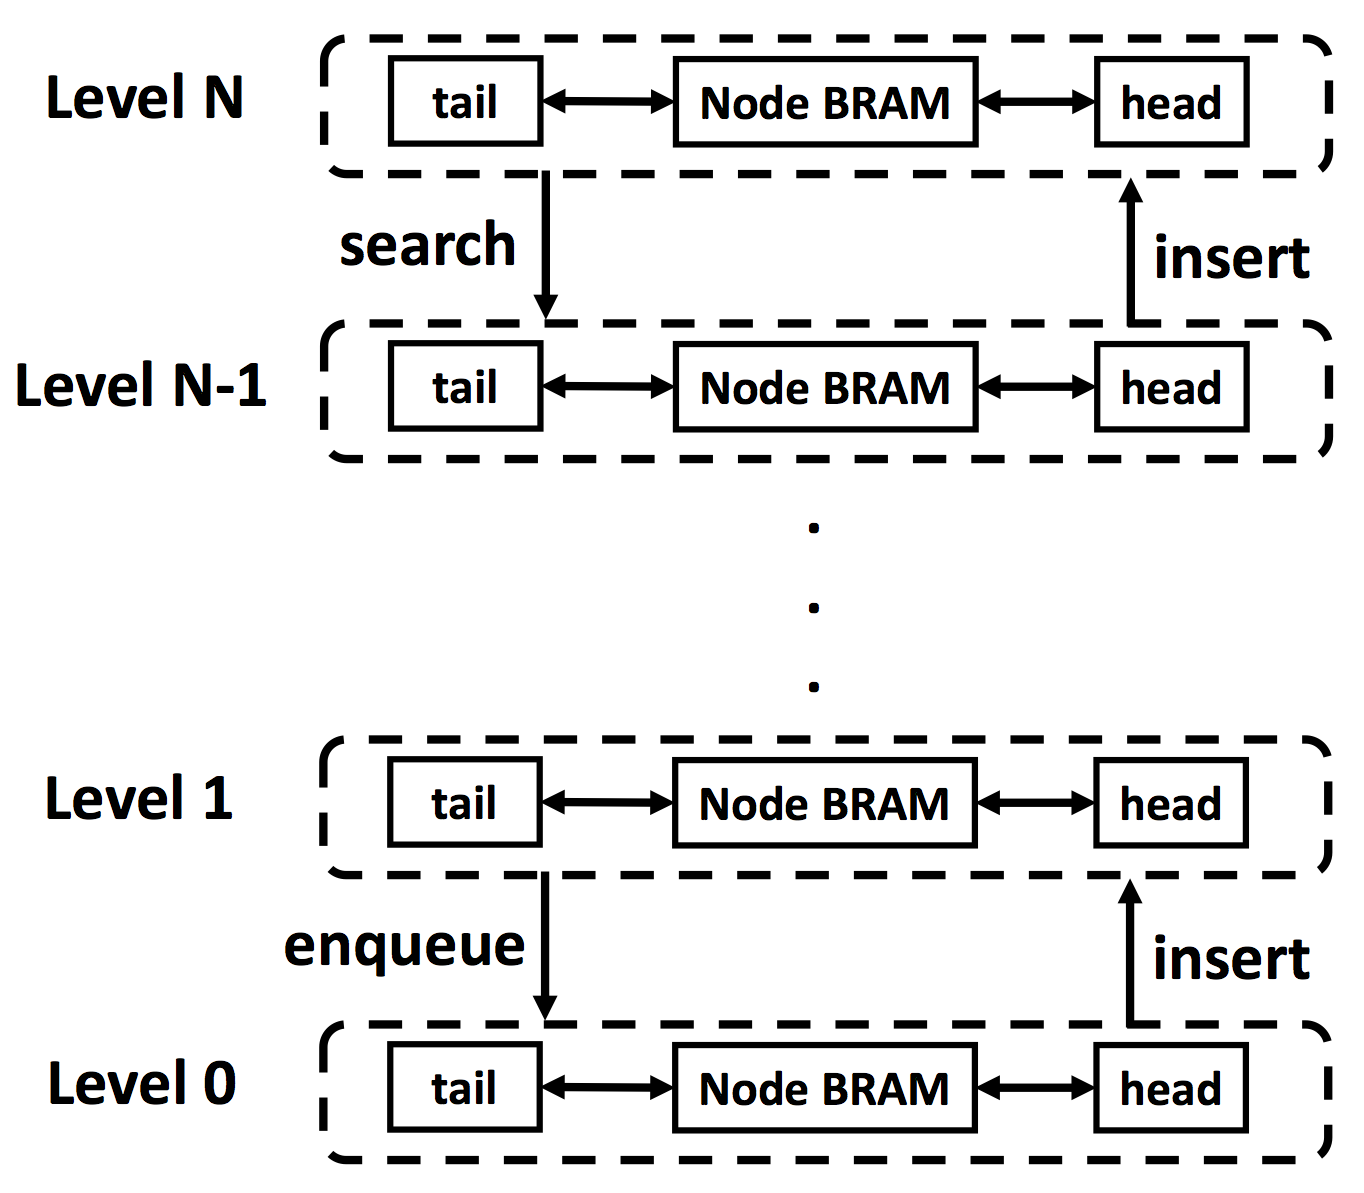
\includegraphics[width=0.8\linewidth]{figures/design/pipe-skip-list}
\caption{Pipelined skip list block diagram.}
\label{fig:pipe-skip-list}
\end{figure}


\subsection{Considerations for Future Scheduler Designs}
In order to make a real production scheduler programmable, one must take into consideration a number of additional features that we have not yet discussed in this paper.

\subsubsection*{Programmability of the Rank Computation}
During the evaluations presented in Section \ref{sec:sched-evals}, we assumed that the rank of each packet was correctly precomputed before arriving at the scheduler. A truly programmable scheduler must allow a developer to express that rank computation in a high-level way; for example, by writing a P4 program. Exactly how the rank computation should interact with the scheduler is non-obvious because it should take place after deciding whether or not to drop the packet. We believe that the P4 language will need to be extended to support a new type of architectural element that will facilitate the implementation of scheduling algorithms.

\subsubsection*{Hierarchical Scheduling Algorithms}
This paper only considers implementing algorithms for which the scheduling order of buffered packets does not change with arrival of future packets. This is consistent with the limitations on the sorts of algorithms that can be implemented using a single PIFO. However, as explained in \cite{pifo2016}, multiple PIFOs can be combined in a tree structure to facilitate the implementation of hierarchical scheduling algorithms, which can in fact cause reordering of packets that are already buffered. When combined into a tree, those PIFOs at the leaf positions store packet descriptors and all other PIFOs store pointers to one of their PIFO children. To enqueue a packet into a PIFO tree, it is first enqueued into the leaf PIFO and then a pointer to the current PIFO is enqueued into the parent all the way up to the root. A dequeue operation proceeds in exactly the opposite direction. Our PIFO design can be wired together into a tree structure, although additional consideration is needed to ensure that the full design will still be able to achieve line rate performance. A naive implementation would simply pipeline the various PIFO enqueue and dequeue operations, although this then requires multiple levels of bypass to ensure that recently enqueued packets can be immediately dequeued if necessary.

\subsubsection*{Non-Work-Conserving Scheduling Algorithms}
The authors of \cite{pifo2016} also discuss the idea of using an additional "shaping" PIFO to implement scheduling algorithms that require input rate limiting. These scheduling algorithms are non-work-conserving and specify the time at which packets should be enqueued, so they require an additional computation to determine this time, what the authors call a "shaping transaction". Presuming that this shaping transaction exists, we believe that our design can be easily extended with a mechanism that examines the current wall clock time before removing an element from the PIFO. This would help to facilitate the implementation of these non-work-conserving algorithms.


\subsubsection*{Alternate Drop Policies}
The design proposed in this paper implements the simplest, and most common, drop policy - tail drop. When using this policy, if an arriving packet encounters a full queue, it is dropped. There are also many other active queue management policies such as RED~\cite{red}, WRED~\cite{wred}, and REM~\cite{rem}. In particular, the one that we believe is most fitting for a PIFO implementation is to enqueue all arriving packets and then drop the one with the lowest priority (highest rank) if the queue exceeds a certain threshold. Dropping packets that are already in the buffer can be challenging, but we believe that it is feasible by extending our design to track the pointer to the head segment of packet with the lowest rank in each queue so that it can be removed if the queue reaches saturation.

\subsubsection*{Broadcasting and Multicasting}
A production scheduler implementation must be capable of supporting broadcasting and multicasting.  These can be implemented by modifying the packet buffer to support replication of packets to all or a subset of the output ports.

% \todo[inline]{Targeting an ASIC}





